%************************************************
% Einleitung
%************************************************
\chapter{Einleitung}
\label{sec:intro}

Mehr als 90 Prozent der Befragten im Alter von 14 bis 29 Jahren sind der Meinung, dass Programmierfähigkeiten vielfältige Möglichkeiten eröffnen, die Welt von Morgen mitzugestalten~\cite{statista-1}. Auch in der Politik wird in Zeiten der Digitalisierung die Forderung nach der Vermittlung von Programmierfähigkeiten für alle Schüler\footnote{Aus Gründen der Lesbarkeit werden Personengruppen in einer Form bezeichnet, wobei immer sowohl weibliche als auch männliche Personen gemeint sind.} immer lauter. Die daraus resultierende Aufgabe stellt Lehrer vor große Herausforderungen. Klassische Programmiersprachen wie Java oder Python bringen einen großen Sprachumfang mit, der Anfänger schnell überfordert~\cite{ko2004}. Simple Eingabe-Ausgabe-Programme, wie sie in diesen Sprachen oft zur Einführung entwickelt werden, da die Einarbeitung in komplizierte Grafik-Bibliotheken selbst für erfahrene Entwickler in der Regel eine recht steile Lernkurve mit sich bringt, demotivieren die Schüler direkt am Anfang~\cite[63]{resnick2009}.

Aus diesem Grund wurden Anwendungen geschaffen, die Anfänger beim Einstieg in die Programmierung unterstützen sollen. Viele dieser Anwendungen, wie z.~B. die Turtle Grafiken (siehe \ref{sec:related:turtle}), erwarten aber weiterhin die Eingabe von getipptem Programmcode, der sich an bestimmte Regeln -- die sogenannte Syntax -- halten muss, damit er ausgeführt werden kann. Auch das Wissen, an welchen Stellen, welcher Befehl einzusetzen ist, muss zunächst gelernt werden. Diese Einstiegshürden führen dazu, dass Schüler schnell das Interesse am Programmieren verlieren~\cite{ko2004}.

Andere Anwendungen versuchen, dies zu vermeiden, indem sie mit syntaxfreier Programmierung wie z.~B. Lightbot (siehe \ref{sec:related:lightbot}) den Code hinter bunten Blöcken und Grafiken verstecken. Dieser Ansatz kann Syntaxfehlern entgegenwirken und die Schüler mit schnell sichtbaren Ergebnissen motivieren. Durch eine Abstraktion der Programmierkonzepte erschweren sie allerdings den späteren Umstieg auf eine echte Programmiersprache~\cite{gouws2013}.

Marcus Riemer liefert mit seiner Masterarbeit BlattWerkzeug einen Ansatz, die Lücke dazwischen zu schließen. Er entwickelte eine Anwendung, welche es Anfängern ermöglicht, Programme mit der Maus aus Blöcken zusammenzustellen, dabei die Anmutung von Programmcode allerdings nicht verschleiert und so die Vorteile beider Vorgehensweisen unter einem Dach zusammenbringt. BlattWerkzeug bietet dank der syntaxfreien Programmierung einen unterstützenden Einstieg, führt dem Neuling aber von Anfang an den Code vor Augen.

Bisher beschränkte sich BlattWerkzeug jedoch auf die Programmierung von Datenbankabfragen und die Zusammenstellung einfacher Bedienoberflächen. Diese Bachelorarbeit beschäftigt sich nun mit der Konzeption und Implementierung einer Erweiterung der Plattform um eine Minisprache -- einer Programmiersprache mit reduziertem Sprachumfang -- welche Neulinge an die Grundkonzepte des Programmierens heranführen soll. In einer Mikrowelt, einer Art virtuellem Spielfeld, sind mit den selbst gebauten Programmen kleine Puzzle Rätsel zu lösen, wodurch die Ausführung der Programmbefehle sichtbar gemacht wird.

Das Kapitel \ref{sec:basics} führt in die für diese Arbeit benötigten Grundlagen ein. Im Kapitel \ref{sec:related} werden anschließend vergleichbare Arbeiten vorgestellt, welche dieser Arbeit als Inspiration gedient haben. Die vorgestellten Arbeiten sind chronologisch ihrer Entstehung nach geordnet und zeichnen so auch den Werdegang dieses Genres auf.

Kapitel \ref{sec:requirements} stellt Anforderungen an die entwickelte Software, welche sich aus den Anforderungen an die im Grundlagenkapitel erläuterten Minisprachen und Mikrowelten aus der Literatur, des bestehenden BlattWerkzeug-Projektes und der Aufgabenstellung bei der Vergabe dieses Themas ergeben.

Die Umsetzung dieser Anforderungen und die damit verbundenen Entscheidungen zu Vorgehensweisen, Softwarearchitektur und eingesetzten technischen Methoden werden in Kapitel \ref{sec:implementation} dargestellt. Im Fazit werden die Anforderungen den erreichten Zielen gegenübergestellt und ein Ausblick gegeben, durch welche Erweiterungen das Ergebnis dieser Arbeit in Zukunft noch weiter verbessert werden könnte.

% \begin{figure}[H]
%   \begin{subfigure}[b]{0.30\textwidth}
%     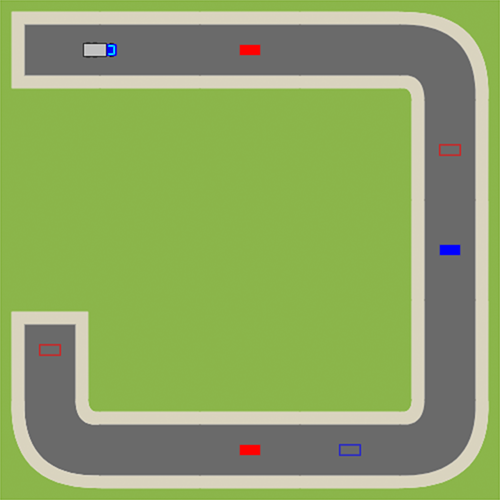
\includegraphics[width=\textwidth]{gfx/exercises-world-d.png}
%     \caption{Beispiel einer Mikrowelt}
%   \end{subfigure}\hfill
%   \begin{subfigure}[b]{0.30\textwidth}
%     \includegraphics[width=\textwidth]{gfx/exercises-program-5.png}
%     \caption{Beispiel eines Programms, welches die Welt löst}
%   \end{subfigure}\hfill
%   \caption{Beispiel Mikrowelt und Minisprache}
% \end{figure}
